\documentclass[11pt,a4paper]{article}

% ---------- Packages ----------
\usepackage[a4paper,margin=2.1cm,top=2.6cm,bottom=2.4cm]{geometry}
\usepackage[utf8]{inputenc}
\usepackage[T1]{fontenc}
\usepackage{helvet}
\renewcommand{\familydefault}{\sfdefault}
\usepackage{microtype}
\usepackage{xcolor}
\usepackage{tikz}
\usetikzlibrary{shapes.geometric,arrows.meta,positioning,fit,backgrounds}
\usepackage{tcolorbox}
\tcbuselibrary{skins}
\usepackage{enumitem}
\setlist{nosep, leftmargin=1.35em, topsep=1pt, itemsep=1.5pt}
\usepackage{titlesec}
\usepackage{fancyhdr}
\usepackage{booktabs}
\usepackage{array}
\usepackage{colortbl}
\usepackage{tabularx}
\usepackage{hyperref}
\usepackage{ragged2e}
\usepackage{multicol}
\usepackage{lastpage}

% ---------- Palette (matches the FOCP platform UI) ----------
\definecolor{focpgreen}{HTML}{1B4332}
\definecolor{focpgreendark}{HTML}{123024}
\definecolor{focpgreenlight}{HTML}{2D6A4F}
\definecolor{focpgold}{HTML}{C9A227}
\definecolor{focpgoldlight}{HTML}{F3E7C4}
\definecolor{focpgray}{HTML}{5B6B63}
\definecolor{focpbg}{HTML}{F7F6F2}
\definecolor{focpline}{HTML}{DDE3DE}

\hypersetup{colorlinks=true, linkcolor=focpgreen, urlcolor=focpgreen}

% ---------- Section styling ----------
\titleformat{\section}
  {\large\bfseries\color{focpgreen}}
  {\thesection.}{0.45em}{}
\titlespacing*{\section}{0pt}{9pt}{5pt}
\titleformat{\subsection}
  {\normalsize\bfseries\color{focpgreenlight}}
  {\thesubsection}{0.4em}{}
\titlespacing*{\subsection}{0pt}{6pt}{3pt}

% ---------- Header / Footer ----------
\pagestyle{fancy}
\setlength{\headheight}{14pt}
\fancyhf{}
\renewcommand{\headrulewidth}{0.6pt}
\renewcommand{\footrulewidth}{0.4pt}
\fancyheadoffset{0pt}
\lhead{\small\color{focpgray}\textbf{Fondation OCP} — Axe Éco-Social}
\rhead{\small\color{focpgray}Cahier des charges — Plateforme FOCP}
\lfoot{\small\color{focpgray}Direction de la Transformation Digitale}
\cfoot{\small\color{focpgray}\thepage / \pageref{LastPage}}
\rfoot{\small\color{focpgray}Confidentiel — usage interne}

\setlength{\parindent}{0pt}
\setlength{\parskip}{2pt}

% ---------- FOCP logo (vector, drawn in TikZ) ----------
\newcommand{\focplogo}[1][0.62]{%
  \begin{tikzpicture}[scale=#1, every node/.style={transform shape}]
    \fill[focpgreen, rounded corners=3pt] (0,0) rectangle (1.15,1.15);
    \fill[focpgold] (0.82,0.18) circle (0.10);
    \node[white, font=\bfseries\fontsize{22}{22}\selectfont] at (0.5,0.62) {F};
  \end{tikzpicture}%
}

\newtcolorbox{infobox}{
  colback=focpbg, colframe=focpline, boxrule=0.5pt, arc=2pt,
  left=6pt, right=6pt, top=4pt, bottom=4pt
}

\newcolumntype{Y}{>{\RaggedRight\arraybackslash}X}

\begin{document}
\thispagestyle{empty}

% ---------- Cover band ----------
\begin{tcolorbox}[
    colback=focpgreen, colframe=focpgreen, arc=3pt,
    left=14pt, right=14pt, top=12pt, bottom=12pt, boxrule=0pt
]
\begin{minipage}[c]{0.14\textwidth}
  \focplogo[0.9]
\end{minipage}%
\begin{minipage}[c]{0.86\textwidth}
  {\color{white}\LARGE\bfseries Cahier des Charges} \\[2pt]
  {\color{focpgoldlight}\large Plateforme de Gestion des Bénéficiaires — Axe Éco-Social} \\[1pt]
  {\color{white!85!focpgreen}\small Fondation OCP\,/\,UM6P — Direction de la Transformation Digitale \quad$\vert$\quad Version 1.0 — Prêt pour développement}
\end{minipage}
\end{tcolorbox}

\vspace{4pt}

\section{Contexte et définition du projet}
La Fondation OCP déploie, à travers son \textbf{Axe Éco-Social}, un réseau national de près de
\textbf{1\,700 coopératives} regroupant des dizaines de milliers de bénéficiaires directs et indirects
à travers le Royaume. Le suivi de ce réseau — bénéficiaires, indicateurs ESG, Objectifs de
Développement Durable (ODD), rapports d'activité, conventions de partenariat et documents
justificatifs — repose aujourd'hui sur des fichiers dispersés (tableurs, échanges par e-mail,
documents papier), non connectés entre eux, difficiles à consolider et à fiabiliser dans le temps.

Ce cahier des charges définit les spécifications fonctionnelles et techniques d'une
\textbf{plateforme décisionnelle centralisée} permettant à la Fondation de piloter l'ensemble du
réseau de coopératives depuis une interface unique, tout en donnant à chaque coopérative un accès
restreint et sécurisé à ses propres données.

\section{Objectifs de la plateforme}
\begin{itemize}
  \item Centraliser les données de \textbf{~1\,700 coopératives} : profils, bénéficiaires, ODD, ESG, documents, conventions.
  \item Fournir à l'administrateur des \textbf{tableaux de bord} et une cartographie interactive pour piloter le réseau national.
  \item Permettre à chaque coopérative de \textbf{saisir et suivre} ses propres statistiques mensuelles et rapports d'activité.
  \item Digitaliser le \textbf{workflow de validation} (soumission → revue → approbation/rejet → notification).
  \item Garantir la \textbf{traçabilité} et la fiabilité des données dans le temps (historisation mensuelle, journal d'audit).
  \item Produire des \textbf{exports} (CSV, Excel, PDF) exploitables par les équipes de reporting internes.
\end{itemize}

\section{Description fonctionnelle de la plateforme}
La plateforme s'articule autour de deux espaces applicatifs — un espace \textbf{Administrateur}
(vision globale du réseau, validation, analytique) et un espace \textbf{Coopérative} (saisie et suivi
limités à l'entité concernée) — reliés à un socle commun de données structurées par commune,
province, région et secteur d'activité.

\begin{center}
\small
\renewcommand{\arraystretch}{1.18}
\begin{tabularx}{\textwidth}{@{}l Y c@{}}
\toprule
\rowcolor{focpgreen}
\textcolor{white}{\textbf{Module}} & \textcolor{white}{\textbf{Fonction}} & \textcolor{white}{\textbf{Espace}} \\
\midrule
Authentification & Connexion par rôle, sessions sécurisées, redirection automatique & Admin / Coop. \\
\rowcolor{focpbg} Tableaux de bord & KPI réseau, évolution mensuelle, répartition par ODD & Admin / Coop. \\
Profil coopérative & Informations générales, localisation, secteur, statut légal & Admin / Coop. \\
\rowcolor{focpbg} Bénéficiaires & Saisie mensuelle (femmes, hommes, jeunes, handicap, indirects) & Coopérative \\
Rapports mensuels & Soumission d'activité, validation/rejet avec commentaire & Admin / Coop. \\
\rowcolor{focpbg} Documents & Téléversement, catégorisation, versioning, revue & Admin / Coop. \\
Import CSV & Import en masse de coopératives, validation ligne par ligne & Admin \\
\rowcolor{focpbg} Carte interactive & Localisation des coopératives, filtres région/secteur/ODD & Admin \\
ODD \& conventions & Association multi-ODD, suivi des conventions et échéances & Admin \\
\rowcolor{focpbg} Recherche avancée & Filtres combinés (nom, région, secteur, statut, ODD) & Admin \\
Notifications & Alertes évènementielles (rapport, document, convention) & Admin / Coop. \\
\rowcolor{focpbg} Analytique \& exports & Graphiques transversaux ; export CSV / Excel / PDF & Admin \\
\bottomrule
\end{tabularx}
\end{center}

\section{Architecture cible de la plateforme}
L'architecture retenue est une architecture web modulaire à trois niveaux, hébergeable sur une
infrastructure cloud standard, conçue pour évoluer sans rupture vers la charge complète du réseau
(1\,700 coopératives).

\begin{center}
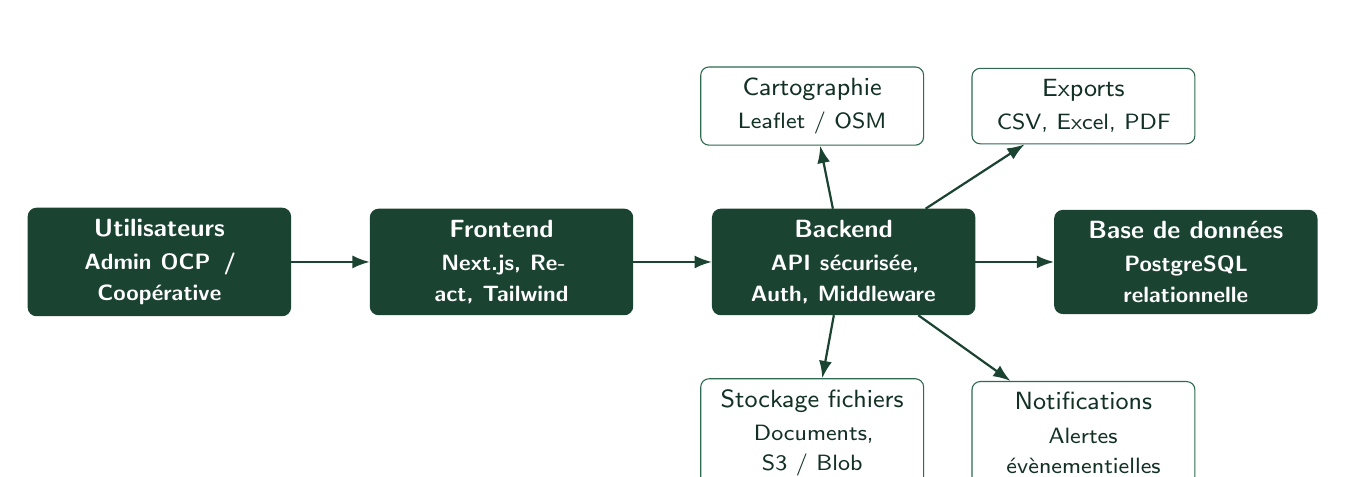
\begin{tikzpicture}[
  font=\small,
  node distance=8mm and 10mm,
  box/.style={rectangle, rounded corners=3pt, draw=focpline, fill=focpbg,
    text width=3.05cm, align=center, minimum height=0.95cm, inner sep=4pt,
    text=focpgreendark, font=\small},
  main/.style={box, fill=focpgreen, text=white, draw=focpgreen, font=\small\bfseries},
  side/.style={box, fill=white, draw=focpgreenlight, text width=2.55cm},
  arr/.style={-{Latex[length=2.2mm]}, focpgreen, thick},
]
  \node[main] (users) {Utilisateurs\\[1pt]\footnotesize Admin OCP \,/\, Coopérative};
  \node[main, right=of users] (frontend) {Frontend\\[1pt]\footnotesize Next.js, React, Tailwind};
  \node[main, right=of frontend] (backend) {Backend\\[1pt]\footnotesize API sécurisée, Auth, Middleware};
  \node[main, right=of backend] (db) {Base de données\\[1pt]\footnotesize PostgreSQL relationnelle};

  \node[side, above=8mm of backend, xshift=-4mm] (map) {Cartographie\\[1pt]\footnotesize Leaflet / OSM};
  \node[side, right=6mm of map] (export) {Exports\\[1pt]\footnotesize CSV, Excel, PDF};
  \node[side, below=8mm of backend, xshift=-4mm] (storage) {Stockage fichiers\\[1pt]\footnotesize Documents, S3 / Blob};
  \node[side, right=6mm of storage] (notif) {Notifications\\[1pt]\footnotesize Alertes évènementielles};

  \draw[arr] (users) -- (frontend);
  \draw[arr] (frontend) -- (backend);
  \draw[arr] (backend) -- (db);
  \draw[arr] (backend) -- (map);
  \draw[arr] (backend) -- (export);
  \draw[arr] (backend) -- (storage);
  \draw[arr] (backend) -- (notif);
\end{tikzpicture}
\end{center}
\vspace{-2pt}
{\footnotesize\color{focpgray}\textit{Flux principal : Utilisateurs $\rightarrow$ Frontend $\rightarrow$ Backend (authentification, règles métier, validation) $\rightarrow$ Base de données ; services associés : cartographie, génération d'exports, stockage documentaire et notifications, tous orchestrés par le backend.}}

\section{Spécifications techniques}
\begin{center}
\small
\renewcommand{\arraystretch}{1.15}
\begin{tabularx}{\textwidth}{@{}l Y@{}}
\toprule
\rowcolor{focpgreen}
\textcolor{white}{\textbf{Composant}} & \textcolor{white}{\textbf{Technologie recommandée}} \\
\midrule
Frontend & Next.js (App Router), React, TypeScript, Tailwind CSS \\
\rowcolor{focpbg} Backend & API sécurisée intégrée (Server Actions / routes API), middleware d'autorisation \\
Base de données & PostgreSQL (production) via ORM relationnel typé \\
\rowcolor{focpbg} Authentification & Sessions signées (JWT en cookie \texttt{httpOnly}), hachage des mots de passe \\
Cartographie & Leaflet / OpenStreetMap, marqueurs géolocalisés et filtres \\
\rowcolor{focpbg} Graphiques & Bibliothèque de visualisation (courbes, barres, aires, camemberts) \\
Stockage documentaire & Service de stockage objet (S3 ou équivalent) \\
\rowcolor{focpbg} Exports & Génération native CSV, Excel (mise en forme), PDF (rapport de synthèse) \\
Hébergement & Environnement cloud avec CI/CD, séparation staging / production \\
\bottomrule
\end{tabularx}
\end{center}

\section{Exigences de sécurité}
\begin{infobox}
\begin{multicols}{2}
\begin{itemize}
  \item Authentification par rôle (Administrateur / Coopérative) avec accès strictement scopé à l'entité concernée.
  \item Mots de passe hachés (bcrypt ou équivalent) ; aucun secret stocké en clair.
  \item Sessions signées, cookies \texttt{httpOnly} / \texttt{sameSite}, expiration automatique.
  \item Middleware de protection sur toutes les routes sensibles (\texttt{/admin}, \texttt{/cooperative}).
  \item Validation systématique des entrées (formulaires, import CSV) côté serveur.
  \item Journal d'audit des actions sensibles (connexion, validation, import, export).
  \item Chiffrement des échanges en transit (HTTPS/TLS obligatoire en production).
  \item Limitation de débit (\emph{rate limiting}) sur les endpoints d'authentification et d'import.
  \item Contrôle d'accès aux documents téléversés (vérification type/taille de fichier).
  \item Sauvegardes régulières de la base de données et procédure de restauration testée.
\end{itemize}
\end{multicols}
\end{infobox}

\section{Livrables et planning de développement}
\begin{center}
\small
\renewcommand{\arraystretch}{1.2}
\begin{tabularx}{\textwidth}{@{}l Y c@{}}
\toprule
\rowcolor{focpgreen}
\textcolor{white}{\textbf{Phase}} & \textcolor{white}{\textbf{Contenu}} & \textcolor{white}{\textbf{Durée indic.}} \\
\midrule
1. Cadrage & Validation du cahier des charges, maquettes, modèle de données & 1 semaine \\
\rowcolor{focpbg} 2. Socle technique & Authentification, base de données, architecture, environnements & 1 semaine \\
3. Modules cœur & Coopératives, bénéficiaires, rapports, documents, workflow de validation & 2 semaines \\
\rowcolor{focpbg} 4. Modules avancés & Carte interactive, import CSV, analytique, exports, notifications & 2 semaines \\
5. Recension \& sécurité & Tests fonctionnels, revue de sécurité, données de démonstration & 1 semaine \\
\rowcolor{focpbg} 6. Mise en production & Déploiement, formation des utilisateurs, documentation & 1 semaine \\
\bottomrule
\end{tabularx}
\end{center}

\textbf{Livrables attendus :} code source documenté, schéma de base de données, jeu de données de
démonstration, guide d'installation, identifiants de démonstration, documentation utilisateur et
feuille de route d'évolution (V2).

\vspace{4pt}
{\footnotesize\color{focpgray}\textit{Ce document constitue la base contractuelle du développement de la plateforme FOCP ;
toute évolution de périmètre fera l'objet d'un avenant validé par la Direction de la Transformation
Digitale de la Fondation OCP.}}

\end{document}
